\section{Задача обновления информации}

После того, как книги найдены и добавлены в базу данных, требуется все время поддерживать ее в рабочем состоянии, обновлять имеющуюся инфомацию и производить поиск дополнительной. Для решения задачи обновления и пополнения базы данных реализован поиск информации на внешних ресурсах, классификация книг на основе аннотации, поиск информации внутри отдельной книги.

\subsection{Задача определения жанра книги}

На сервере хранится база данных, заполненная собранной в Интернете информацией о книгах. В информацию о книге входят --- название, автор, описание, жанр и некоторые другие поля. Обязательными для книги являются название книги и автор (у каждой книги может быть указано больше одного автора). Для некоторых книг в найденной информации уже указан жанр, для других --- нет. 

Для более удобной навигации пользователя по базе, сервер предоставляет возможность различных выборок, в том числе по жанру, но для многих книг анализатор не может определить жанр, исходя из информации, находящейся на той странице, где была найдена книга. Для предоставления пользователю более полной информации реализовано определение жанра книги, исходя из её аннотации. 

Для реализации были использованы техники искусственного интеллекта, а именно машинного обучения. Машиное обучение \cite{machine-learning} --- это обширный подраздел искусственного интеллекта, изучающий методы построения алгоритмов, способных обучаться. В большинстве случаев это означает, что алгоритму подается на вход набор данных, а он выводит информацию о свойствах этих данных, причем так, что на основе выведенной информации способен делать предсказания о данных, которые может увидеть в будущем. Это возможно потому, что практически все неслучайные данные содержат какие-то закономерности (паттерны) и, выявив их, машина способна сделать обобщение. У машинного обучения есть свои слабости. Алгоритмы различаются по способности делать обобщения на основе больших наборов паттернов, и если некий паттерн никогда прежде не встречался, то возможна его ошибочная интерпретация. Природа алгоритмов машинного обучения такова, что они продолжают обучаться по мере поступления новой информации.

Для реализации определения жанра книги рассматривались многие возможности машинного обучения, а именно методы обучения с учителем, такие как Байесовский классификатор, деревья решений, нейронные сети, метод k-средних и пр. \cite{collective-intelligence}

Классификатор, построенный на основе деревьев решений, не поддерживает инкрементальное обучение. Так же, для больших наборов данных дерево может оказаться слишком большим, что существенно замедлит процесс классификации. Нейронные сети, в свою очередь, поддерживают инкрементальное обучение, но являются своего рода <<черным ящиком>>. В реальных сетях имеются сотни нейронов и тысячи синапсов, поэтому понять как сеть выбрала ответ невозможно, что делает невозможным более тонкую ручную настройку классификатора. Основным недостатком метода k-средних является то, что для прогнозирования ему требуются все данные, на которых производилось обучение. На это расходуется не только память, но и время --- для выработки каждого прогноза приходится сравнивать новый образец с каждым из имеющихся, чтобы найти ближайшие. 

В итоге проведенного анализа алгоритмов, для реализации был выбран Байесовский классификатор, как наиболее подходящий для обучения и опрашивания на больших наборах данных. Даже если обучающий набор очень велик, обычно для каждого образца есть лишь небольшое количество признаков, а обучение и классификация сводятся к простым математическим операциям над вероятностями признаков. Важной особенностью такого классификатора является возможность инкрементного обучения, \te каждый новый предъявленный образец можно использовать для обновления вероятностей без использования старых обучающих данных. Поддержка инкрементного обучения важна, \tk это дает возможность классификатору обучаться на вновь поступающих в базу данных книгах. Классификатор должен обновляться быстро и без дополнительных запросов к базе данных о книгах, на которых был обучен. Ещё одно достоинство наивного Байесовского классификатора --- относительная простота интерпретации того, чему классификатор обучился. Это позволяет более точно настраивать полученный классификатор, изменяя вероятности для некоторых признаков.

Наивный байесовский классификатор это простой вероятностный классификатор, основанный на применении Теоремы Байеса со строгими (наивными) предположениями о независимости. Для определения вероятности для всего документа был выбран метода Фишера \cite{collective-intelligence}. 
В отличие от наивной байесовсой фильтрации, когда для вычисления вероятности всего документа перемножаются вероятности отдельных признаков, по методу Фишера вычисляется вероятность отнесения к той или иной категории для каждого признака документа, после чего эти вероятности комбинируются и проверяется, насколько получившееся множество похоже на случайное. Хотя этот метод более сложен, он обеспечивает большую гибкость при настройке параметров классификации.

В качестве входа классификатор принимает текст. Этот текст разбивается на слова. Каждое слово подвергается стеммингу. Стемминг \cite{stemming} --- это процесс нахождения основы слова для заданного исходного слова. Основа слова необязательно совпадает с морфологическим корнем слова. В итоговый вектор добавляются все слова и пары слов, встреченные в тексте.

\begin{figure}
\centering
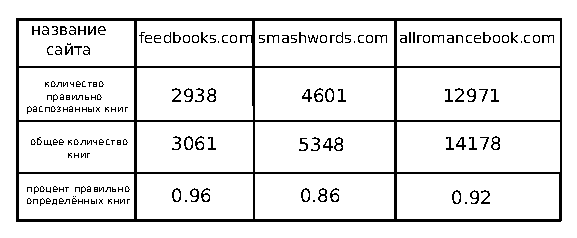
\includegraphics[width=.7\textwidth]{./statistics}
\caption{Таблица успешности распознавания жанра книги.}\label{fig:scheme1}
\end{figure}

В случае классификации книг, в качестве входа использовались название книги и ее аннотация. В том случае, если описание еще не хранилось базе данных происходил поиск описания на Amazone\cite{amazon}.

Перед первым проходом классификатора, определяющего жанры книг запускается скрипт, собирающий дополнительную информацию об авторах. Такой информацией являются жанры, в которых пишет автор. Поиск такого рода информации происходит на внешних ресурсах. В основном, используется информация с сайта Wikipedia \cite{wiki}. После проведения классификации авторов, запускается скрипт, выполняющий классификацию книг. Во время этой классификации учитывается автор, написавший данную книгу. Для жанров, в которых пишет автор, увеличивается вероятность.

Таким образом, во время классификации частично решается задача поиска дополнительной информации о книгах на внешних ресурсах и задача поиска информации об авторах на внешних ресурсах.

Тестирование классификатора проводилось на ресурсах, предоставляющих информацию о книгах в формате OPDS, таких, как \\ Feedbooks\cite{feedbooks}, AllRomance\cite{allrom}\  и SmashWords\cite{smash}. 

Эти ресурсы были выбраны, т.к. их содержимое не сильно пересекается. На ресурсе Feedbooks основным жанром является Adventures($\sim$60\% книг), наиболее частым для  AllRomance является Romantic\_Literature (так же, $\sim$60\% книг). На ресурсе SmashWords книги более-менее равномерно распределены по жанрам.

В тексте приведена таблица успешности распознавания жанра в зависимости от ресурса(\picref{fig:scheme1}). Из таблицы видно, что среднее количество правильно распознанных книг -- 90 \%. Более низкий уровень распознавания для SmashWords объясняется невысоким качеством предлагаемых аннотаций. Эти аннотации содержат большое количество шумов(таких, как обрывки слов, несвязанные слова в предложении и т.д.). Часть шумов такого рода убирается на этапе добавления слов в итоговый вектор.

\subsection{Поиск информации на внешних ресурсах}

Задача поиска дополнительной информации решается одновременно с решением других задач. Например, поиск аннотации для книг производится во время их классификации по жанрам.
В работе реализован поиск дополнительной информации на сайте Amazon \cite{amazon} --- поиск аннотации для книг, на сайте Wikipedia \cite{wiki} происходит поиск дополнительной информации для авторов(теги).

Для поиска информации о книгах на внешних ресурсах необходимо анализировать большие объемы HTML страниц, \tk пока не существует ресурсов, предоставляющих информацию о большом количестве книг в унифицированном формате. Для обработки страниц использовалась библиотека Beautiful Soup \cite{beaut-soup}. Beautiful Soup --- это написанный на Python анализатор документов в форматах HTML и XML. Он спроектирован так, что способен работать с плохо написанными  веб-страницами. Одновременно с этим, библиотека предоставляет достаточно удобный интерфейс использования.


\subsection{Извлечение информации из форматов epub и fb2}

Для пополнения базы данных так же используется извлечение информации из книг в формате epub и fb2. В случае, если анализатор не смог определить название полученной от <<поискового паука>> книги и ее автора, но найденный файл --- в фомате fb2 или epub, в базу данных добавляется ссылка на этот файл, но эта ссылка не привязывается ни к одной книге. Это делается, \tk из этих форматов можно извлечь нужную информацию. 

Electronic Publication (ePub) \cite{epub} — открытый формат электронных версий книг. Формат позволяет издателям производить и распространять цифровую публикацию в одном файле, обеспечивая совместимость между программным и аппаратным обеспечением, необходимым для воспроизведения незашифрованных цифровых книг и других публикаций с плавающей вёрсткой.
Zip-архив контейнера ePub содержит тексты в форматах xHTML, HTML или PDF, описание издания в XML, рядом в папках — графика, включая векторную (SVG), и встроенные шрифты, таблицы стилей и \td 

FictionBook \cite{fb2} — формат представления электронных версий книг в вие XML-документов, где каждый элемент книги описывается своими тегами. Стандарт призван обеспечить совместимость с любыми устройствами и форматами. XML позволяет легко создавать документы, готовые к непосредственному использованию и программной обработке (конвертации, хранению, управлению) в любой среде. Документы содержат структурную разметку основных элементов текста, некоторое количество информации о книге, а также могут содержать вложения с двоичными файлами, в которых могут храниться иллюстрации или обложка.

Оба фомата хранят информацию о книге в удобном для автоматической обработки формате. Оба формата имеют xml-схему, с помощью корой происходит валидация документа и с помощью которой возможно написать парсер извлекающий нужную информацию.